\documentclass{book}
\usepackage[utf8]{vietnam}
\usepackage{cite}
\usepackage{amsmath,amssymb,amsfonts}
\usepackage{algorithm}
\usepackage{algorithmic}
\usepackage{graphicx}
\usepackage{textcomp}
\usepackage{xcolor}
\usepackage{tabularx}
\usepackage{listings}
\usepackage{enumerate}

\newcounter{savedenum}
\newcommand*{\saveenum}{\setcounter{savedenum}{\theenumi}}
\newcommand*{\resume}{\setcounter{enumi}{\thesavedenum}}


\begin{document}
%\title{TỐI ƯU LỒI VÀ ỨNG DỤNG TRONG MÁY HỌC}
%\author{Võ Thị Lưu Phương}
%
%
%\maketitle

\setcounter{chapter}{4}
\chapter{LÝ THUYẾT ĐỐI NGẪU}
\textit{Tác giả: Võ Thị Lưu Phương\\Email: vtlphuong@hcmiu.edu.vn}


\section{Giới thiệu}
Lý thuyết đối ngẫu là một chủ đề quan trọng trong lĩnh vực tối ưu. Nhiều lúc ta giải bài toán đối ngẫu thay vì bài toán gốc. Xem xét bài toán đối ngẫu giúp thấy được một số ý nghĩa đằng sau các ràng buộc, các biến.

%Trong phần đầu tiên, linear program, tôi đã giới thiệu bài toán đối ngẫu của một bái toán quy hoạch tuyến tính để bạn đọc có một cái nhìn sơ lược về lý thuyết đối ngẫu.
%Với bài toán LP tổng quát:
%\begin{align}
%\mathrm{min.}~ & c^Tx = c_1 x_1 + \ldots + c_2 x_2 \\
%\mathrm{s.t.}~ & a_{j1}x_1+ \ldots + a_{jn}x_n \geq b_j, j=1,\ldots, m\\
%		&	x_1, \ldots, x_n \geq 0.
%\end{align}
%%Nhân hai vế mỗi ràng buộc với một biến và cộng các ràng buộc vế theo vế, ta được
%Bài toán đối ngẫu có dạng:
%\begin{align}
%\mathrm{max.}~ & b^T \lambda = b_1 \lambda_1 + \ldots + b_m \lambda_m \\
%\mathrm{s.t.}~ & a_{1j}\lambda_1+ \ldots + a_{nj}\lambda_n \leq c_j, j=1,\ldots, m\\
%		&	\lambda_1, \ldots, \lambda_m \geq 0.
%\end{align}
%Số lượng biến của bài toán đối ngẫu bằng số lượng ràng buộc của bài toán gốc và số lượng ràng buộc của bài toán đối ngẫu bằng với số lượng biến của bài toán gốc.
%Một tính chất quan trọng là \textbf{nghiệm của bài toán LP đối ngẫu cũng trùng với nghiệm của bài toán LP gốc}. Do đó, thay vì giải bài toán gốc, ta có thể giải bài toán đối ngẫu.

Sau đây tôi sẽ đề cập về lý thuyết đối ngẫu cho một bài toán tối ưu dạng tổng quát. Các nội dung bao gồm hàm Lagrange, bài toán đối ngẫu, điều kiện Karush-Kuhn-Tucker, và một số phân tích liên quan đến đối ngẫu.

\section{Hàm Lagrange}
Xét bài toán tối ưu tổng quát:
\begin{align}
\mathrm{Primal: ~min.} & f_0(x)\\
\mathrm{s.t.} & f_i(x) \leq 0, i = 1, \ldots, m \\
			& h_i(x) = 0, i = 1, \ldots, p.
			\label{optProb}
\end{align}
trong đó $x \in \mathbb{R}^n$, miền xác định $\mathcal{D} = \cap_{i=0}^m \mathbf{dom} f_i \cap \cap_{i=1}^p \mathbf{dom} h_i$ khác rỗng.
Gọi $p^*$ là nghiệm của bài toán.

Hàm Lagrange $L: \mathbb{R}^n \times \mathbb{R}^m \times \mathbb{R}^r$, hay còn gọi là Lagrangian, được định nghĩa như sau: 
\begin{align*}
L(x, \lambda, \nu) = f_0(x) + \sum_{i = 1}^m \lambda_i f_i(x) + \sum_{i = 1}^p \nu_j h_j(x)
\end{align*}
Các biến $\lambda \in \mathbb{R}^m, \lambda \geq 0$ và $\nu \in \mathbb{R}^p$ được gọi là các \textbf{toán tử Lagrange} (Lagrange multiplier), hay \textbf{biến đối ngẫu} (dual variable). $\lambda_i, i=1,...,m$ tương ứng với ràng buộc $f_i (x) \leq 0$ và $\nu_j, j=1,...,r$ tương ứng với ràng buộc $h_j(x) = 0$.

%Lagrangian chính là tổng của objective với các ràng buộc có nhân với trọng số.
Lagrangian là hàm kết hợp tuyến tính giữa mục tiêu và các ràng buộc.
Nếu ta nhìn bài toán tối ưu là tìm $x$ sao cho công ty vận hành với cực tiểu chi phí với các ràng buộc về nguồn lực $f_i$ và $h_i$. Như vậy hàm Lagrange có thể xem như hàm \textbf{chi phí cộng thêm với các chi phí phát sinh khi các nguồn lực bị vượt quá}. 
$\lambda_i$ có thể được xem như là giá (price) cho một đơn vị của nguồn lực $f_i$ vượt quá ngưỡng.

Ta luôn có \textbf{Lagrangian là một chặn dưới của hàm $f_0(x)$} với mọi $x$ thuộc tập khả thi và $\lambda \geq 0$.
\begin{align}
L(x, \lambda, \nu) = f_0(x) + \sum_{i = 1}^m \lambda_i f_i(x) + \sum_{i = 1}^p \nu_j h_j(x) \leq f_0(x).
\label{eq:lagrangian_lowerbound}
\end{align}

\section{Hàm đối ngẫu}
Định nghĩa \textbf{hàm đối ngẫu} (dual) $g: \mathbb{R}^m \times \mathbb{R}^p \rightarrow \mathbb{R}$ là cực tiểu của Lagrangian theo biến $x$
\begin{align*}
g(\lambda, \nu) = \min_{x \in \mathcal{D}} L(x, \lambda, \nu) = \min_{x \in \mathcal{D}} \Big( f_0(x) + \sum_{i = 1}^m \lambda_i f_i(x) + \sum_{i = 1}^p \nu_i h_i(x) \Big)
\end{align*}

Từ tính chất \eqref{eq:lagrangian_lowerbound}, ta có hàm  đối ngẫu là một chặn dưới của nghiệm $p^*$ của bài toán tối ưu Primal \eqref{optProb}: 
\begin{align}
g(\lambda, \nu) \leq p^*, \forall \lambda \geq 0, \nu.
\end{align}

Sau đây là một vài ví dụ tính hàm  đối ngẫu:

\subsection*{Ví dụ 1:} 
\begin{align}
\mathrm{min.~} & x^T x 		\label{prob:quadratic}\\
\mathrm{s.t.~} & Ax = B 
%\label{linearLeastSquare}
\end{align}
trong đó $A \in \mathbb{R}^{p \times n}$.

Hàm Lagrange có dạng 
\begin{align*}
L(x, \nu) = x^T x + \nu^T(Ax - b).
\end{align*} 

Hàm đối ngẫu được cho bởi công thức:
\begin{align*}
g(v) = \min_x L(x, v)
\end{align*}
Cực tiểu đạt tại $\nabla_x L(x, \nu) = 2x + A^T \nu = 0$. Giải phương trình ta được nghiệm $x = -(1/2) A^T \nu$.
Thay $x$ vào hàm Lagrange, ta được hàm đối ngẫu của bài toán \eqref{prob:quadratic}:
\begin{align*}
g(\nu) = -(1/4) \nu^T A A^T \nu - b^T \nu
\end{align*}
Hàm đối ngẫu $g(\nu)$ là một hàm lõm do ma trận $AA^T$ xác định dương. 
Tính chất chặn dưới của hàm $f_0$ có nghĩa rằng $g(\nu) \leq \min\{x^T x | Ax = B\}$.

\subsection*{Ví dụ 2:}
Xét bài toán quy hoạch tuyến tính
\begin{align}
\mathrm{min~} & c^T x \label{prob:lp}\\
\mathrm{s.t.~} & Ax = B \\
			& x \geq 0,
\end{align}
trong đó $x \in \mathbb{R}^n$. 

Trong bài toán trên, ràng buộc bất đẳng thức chính là $f_i(x) = - x_i \leq 0, i = 1, \ldots, n$.

Lagrangian có dạng: 
\begin{align*}
L(x, \lambda, \nu) = c^T x - \sum_{i = 1}^n \lambda_i x_i + \nu^T (Ax - b) = -b^T \nu + (c + A^T \nu - \lambda)^T x.
\end{align*}

Hàm đối ngẫu của bài toán trên có dạng: 
\begin{align*}
g(\lambda, \nu) &= \min_x L(x, \lambda, \nu) = -b^T \nu + \min_x(c + A^T \nu - \lambda)^T x \\
		& = \begin{cases} -b^T \nu, ~ \textrm{nếu} ~ c + A^T \nu - \lambda = 0 \\ -\infty , ~ \textrm{nếu} ~ c + A^T \nu - \lambda \neq 0 \end{cases}
\end{align*}
Để hàm $g(\lambda, \nu)$ là một chặn dưới có giới hạn của $f_0$ ta cần $\lambda \geq 0$ và $c + A^T \nu - \lambda = 0$.


\section{Liên hợp (đọc thêm)}
Hàm đối ngẫu và liên hợp (conjugate) của hàm $f_0$ có mối liên quan với nhau. Ta có thể tính hàm đối ngẫu từ liên hợp của $f_0$. 
Một số sách về tối ưu hóa như \cite{boyd} thường hay sử dụng liên hợp của hàm để viết hàm đối ngẫu hay bài toán đối ngẫu. Phần này được giới thiệu giúp bạn đọc không cảm thấy bỡ ngỡ khi đọc các tài liệu khác.

Cho hàm $f: \mathbb{R}^n \rightarrow \mathbb{R}$. \textbf{Liên hợp} (conjugate) của hàm $f$, ký hiệu $f^*: \mathbb{R}^n \rightarrow \mathbb{R}$, được định nghĩa là hàm
\begin{align*}
f^*(y) = \max_{x \in \mathbf{dom} f} (y^Tx - f(x)).
\end{align*}

Ta có $f^*$ luôn là một hàm lồi vì nó có dạng là cực đại của các hàm affine theo $y$.

Một số ví dụ về liên hợp:
\begin{itemize}
\item $f(x) = ax + b$: hàm $\max_{x \in \mathbf{dom} f} (yx - ax - b)$ có giới hạn khi và chỉ khi $y = a$. Do đó, miền xác định của hàm liên hợp chỉ là một điểm $\{a\}$, và $f^*(a) = -b$.

\item $f(x) = -\log x, x \in \mathbb{R}$: hàm $\max_x (xy + \log x)$ đạt cực đại tại $x = -1/y$ (với $y < 0$). 
Vì vậy
\begin{align*}
f^*(y) = -\log(-y) - 1, y<0.
\end{align*}

\item $f(x) = x \log x$: $f^*(x) = \max_x (xy - x \log x)$ đạt cực đại tại $x = e^{y-1}$. Vì vậy,
\begin{align*}
f^*(y) = e^{y-1}.
\end{align*}

%\item Log-sum-exp $f(x) = \log(\sum_{i=1}^n e^{x_i})$.
%\begin{align*}
%f^*(y) = \begin{cases} \sum_{i=1}^n y_i \log(y_i) & \textrm{nếu} ~ y \geq 0, 1^Ty = 1 \\
%\infty & otherwise \end{cases}
%\end{align*}

%\item Norm $f(x) = \| x \|$
%\begin{align*}
%f*(y) = \begin{cases} 0 & \textrm{nếu} ~ \|y\|_* \leq 1 \\
%\infty & \|y\|_* \geq 1 \end{cases}
%\end{align*}
\end{itemize}

Cho bài toán tối ưu
\begin{align*}
\mathrm{min~} & f_0(x) \\
\mathrm{s.t.~} & Ax \leq b \\
			& Cx = d.
\end{align*}
Hàm đối ngẫu và hàm liên hợp có liên quan với nhau như sau:
\begin{align*}
g(\lambda, \nu) &= \min_x(f_0(x) + \lambda^T(Ax - b) + \nu ^T(Cx - d)) \\
			& = -b^T \lambda - d^T \nu + \min_{x}(f_0(x) + (A^T \lambda + C^T \nu)^T x) \\
			& = -b^T \lambda - d^T \nu - f^*_0(- A^T \lambda - C^T \nu).
\end{align*}

\subsection*{Ví dụ 3:}
Ví dụ ta có thể tính hàm đối ngẫu trực tiếp từ liên hợp trong bài toán tìm cực tiểu hàm negative entropy:
\begin{align*}
\mathrm{min~} & f_0(x) = \sum_{i = 1}^n x_i \log x_i \\
\mathrm{s.t.~} & Ax \leq b \\
			& 1^T x = 1,
\end{align*}
Trong đó $A$ là ma trận $r \times n$
Ta có
\begin{align*}
g(\lambda, \nu) = -b^T\lambda - \nu - f^*_0(A^T \lambda - \nu)).
\end{align*}
Ta có theo ví dụ phía trên, liên hợp của $f(x) = x\log x$ là $f^*(y) = e^{y-1}$, $y \in \mathbb{R}$.
Do đó, $f_0^*(y) = \sum_{i=1}^n e^{y_i - 1}$. Vì vậy,
\begin{align*}
g(\lambda, \nu)	&= -b^T\lambda -  \nu - \sum_{i = 1}^r  e^{-a_{:,i}^T \lambda - \nu - 1} = -b^T\lambda -  \nu e^{- \nu - 1}\sum_{i = 1}^r e^{-a_{:,i}^T \lambda},
\end{align*}
Trong đó $a_{:,i}$ là cột thứ $i$ của ma trận $A$.



\section{Bài toán đối ngẫu}
Như đã đề cập ở trên, \textbf{hàm đối ngẫu} là một chặn dưới của $p^*$. 
Như vậy \textbf{bài toán đối ngẫu} sau 
\begin{align*}
\mathrm{Dual: ~max.} ~& g(\lambda, \nu) \\
\mathrm{s.t.~} & \lambda \geq 0.
\end{align*}
sẽ cho một chặn dưới tối ưu của bài toán Primal \eqref{optProb}.

Điểm cực trị của bài toán đối ngẫu $(\lambda^*, \nu^*)$ được gọi là \textbf{điểm đối ngẫu tối ưu} (dual optimal), hay \textbf{toán tử Lagrange tối ưu}.

\subsection*{Ví dụ 4:}
%Xét bài toán đã cho ở phần đầu tiên:
Xét bài toán tối ưu:
\begin{align}
\mathrm{min~} & x_1^2 + x_2^2 - 2x_1 \label{eq:ex1_lp}\\
\mathrm{s.t.~} & 2x_1 + x_2 \geq 5 \nonumber\\
			& x_2 \leq 7. \nonumber
\end{align}
Lagrangian được cho bởi công thức:
\begin{align*}
L(x_1, x_2, \lambda_1, \lambda_2) = & x_1^2 + x_2^2 - 2 x_1  \\
								& + (-2x_1 - x_2 + 5)\lambda_1 \\
								& + (x_2 - 7) \lambda_2.
\end{align*}

Hàm đối ngẫu
\begin{align*}
g(\lambda_1, \lambda_2) = & \min_{x_1, x_2} L(x_1, x_2, \lambda_1, \lambda_2) \\
							= & \min_{x_1} x_1^2 - 2(1 + \lambda_1) x_1 \\
								& + \min_{x_2} x_2^2 + (- \lambda_1 + \lambda_2) x_2\\
								& + 5\lambda_1 - 7 \lambda_2. 
\end{align*}

Cực tiểu của $L$ theo $x_1, x_2$ đạt tại:
\begin{align*}
x_1 &= 1 + \lambda_1\\
x_2 &= \frac{1}{2} (\lambda_1 - \lambda_2).
\end{align*}
Do đó hàm đối ngẫu có dạng sau:
\begin{align*}
g(\lambda_1, \lambda_2) &= - (1 + \lambda_1)^2 - \frac{1}{4} (\lambda_1 - \lambda_2)^2 + 5\lambda_1 - 7 \lambda_2.
\end{align*}

\subsection*{Ví dụ 5:}
Xét bài toán LP dạng tổng quát
\begin{align}
\mathrm{min~} & c^T x \label{eq:ex2_lp}\\
\mathrm{s.t.~} & Ax = B \\
			& x \geq 0.
\end{align}

Hàm đối ngẫu được cho bởi: 
\begin{align*}
g(\lambda, \nu) &= \min_x L(x, \lambda, \nu) = -b^T \nu + \min_x(c + A^T \nu - \lambda)^T x \\
		& = \begin{cases} -b^T \nu ~ \textrm{nếu} ~ c + A^T \nu - \lambda = 0 \\ -\infty , \textrm{nếu không} \end{cases}
\end{align*}

$-\infty$ là một chăn dưới đương nhiên của mọi hàm số. Do đó để cho hàm đối ngẫu $g(\lambda, \nu)$ là một chặn dưới thực sự thì ta cần có $c + A^T \nu - \lambda = 0$

Bài toán đối ngẫu của bài toán LP \eqref{eq:ex2_lp} là bài toán tìm chặn dưới tối ưu nhất
\begin{align*}
\max & - b^T \nu \\
\mathrm{s.t.~} & A^T \nu - \lambda + c = 0 \\
			& \lambda \geq 0.
\end{align*}
hay tương dương với
\begin{align*}
\max & - b^T \nu \\
\mathrm{s.t.~} & A^T \nu  + c \geq 0.
\end{align*}

\subsection*{Ví dụ 6:}
Xét bài toán LP có ràng buộc dạng bất đẳng thức:
\begin{align}
\mathrm{min~} & c^T x \label{eq:ex3_lp}\\
\mathrm{s.t.~} & Ax \geq b
\end{align}

Hàm đối ngẫu được cho bởi: 
\begin{align*}
g(\lambda) &= \min_x L(x, \lambda) = -b^T \lambda + \min_x(A^T \lambda + c)^T x \\
		& = \begin{cases} -b^T \lambda ~ \textrm{nếu} ~ A^T + c \lambda = 0 \\ 
		-\infty , ~\textrm{nếu}~ A^T + c \lambda \neq 0 \end{cases}
\end{align*}

Do đó, bài toán đối ngẫu của bài toán \eqref{eq:ex3_lp} có dạng:
\begin{align*}
\max & - b^T \lambda \\
\mathrm{s.t.~} & A^T \lambda + c = 0 \\
			& \lambda \geq 0.
\end{align*}

\section{Tính chất đối ngẫu yếu và mạnh}

\subsection{Đối ngẫu yếu (weak duality)}
Gọi $p^*$ và $d^*$ là giá trị cực trị của bài toán gốc và bài toán đối ngẫu.
Do tính chất hàm đối ngẫu luôn là chặn dưới của $p^*$ nên ta có bất đẳng thức:
\begin{align*}
d^* \leq p^*
\end{align*}
luôn đúng. Bất đẳng thức trên được gọi là \textbf{tính đối ngẫu yếu} của bài toán Primal \eqref{optProb}.
Giá trị $p^* - d^*$ được gọi là khoảng cách đối ngẫu tối ưu (optimal duality gap) của bài toán Primal.

\subsection{Đối ngẫu mạnh (strong duality)}
Trong trường hợp $d^* = p^*$, ta nói bài toán Primal \eqref{optProb} có tính \textbf{đối ngẫu mạnh} (strong duality).
Ta có tính chất sau:
Nếu bài toán Primal \eqref{optProb} lồi và điều kiện Slater thỏa mãn thì bài toán có tính đối ngẫu mạnh.

Điều kiện Slater: tồn tại một điểm trong (interior point) của tập khả thi của bài toán,
hay còn có nghĩa là tồn tại một điểm $x \in \mathbf{relint} \mathcal{D}$ sao cho $f_i(x) < 0, i = 1, \ldots, m$ và $Ax = b$.


\section{Các điều kiện tại điểm cực trị}

\subsection{Complementary slackness}
Một số tài liệu kinh tế dịch complementary slackness là định lý bù yếu.
Giả sử bài toán tối ưu có tính đối ngẫu mạnh, tức là
\begin{align*}
f_0(x^*) & = g(\lambda^*, \nu^*)
\end{align*}
Tuy nhiên ta có:
\begin{align*}
g(\lambda^*, \nu^*)	& = \min_x \Big( f_0(x) + \sum_{i = 1}^m \lambda_i^* f_i(x) + \sum_{i = 1}^p \nu_i^* h_i(x) \Big)\\
	& \leq f_0(x^*) + \sum_{i = 1}^m \lambda_i^* f_i(x^*) + \sum_{i = 1}^p \nu_i^* h_i(x^*) \\
	& \leq f_0(x^*).
\end{align*}

Từ đó dẫn đến $\sum_{i = 1}^m \lambda_i^* f_i(x^*) = 0$. 
Do đó
\begin{align}
\lambda_i^* f_i(x^*) = 0, \forall i = 1, \ldots, m.
\end{align}

\textbf{Nếu $\lambda_i^* > 0$, thì $f_i(x^*) = 0$ (ràng buộc $i$ chặt tại $x^*$) và nếu $f_i(x^*) < 0$ (ràng buộc $i$ lỏng tại $x^*$), thì $\lambda_i^* = 0$.}


\subsection{Điều kiện Karush-Kuhn-Tucker}

Giả sử hàm mục tiêu và các hàm ràng buộc $f_0, \ldots, f_m, h_1, \ldots, h_p$ khả vi.
Gọi $x^*$ và $(\lambda^*, \nu^*)$ lần lượt là các điểm cực trị của bài toán chính và bài toán đối ngẫu.
Nếu ta có đối ngẫu mạnh thì các điều kiện \textit{Karush-Kuhn-Tucker (KKT)} thỏa mãn:
\begin{align}
f_i(x^*) & \leq 0, i = 1, \ldots , m \label{eq:kkt1}\\
h_i(x^*) & = 0, i = 1, \ldots , p \label{eq:kkt2}\\
\lambda_i^* & \geq 0, i = 1, \ldots , m \label{eq:kkt3}\\
\lambda_i^* f_i(x^*) & = 0, i = 1, \ldots , m \label{eq:kkt4}\\
\nabla f_0(x^*) + \sum_{i = 1}^m \lambda_i^* \nabla f_i(x^*) + \sum_{i = 1}^p \nu_i^* \nabla h_i(x^*) & = 0. \label{eq:kkt5}
\end{align}

Hai điều kiện đầu tiên \eqref{eq:kkt1}-\eqref{eq:kkt2} là điều kiện cho $x^*$ là một điểm hợp lệ trong tập khả thi của bài toán Primal.
Điều kiện \eqref{eq:kkt3} là điều kiện cho $\lambda^*$ là một điểm hợp lệ trong tập khả thi của bài toán Dual.
Điều kiện \eqref{eq:kkt4} chính là complementary slackness.
Điều kiện \eqref{eq:kkt5} chính là $\nabla_x L = 0$. 

Trong trường hợp bài toán chính là tối ưu lồi, các điều kiện KKT cũng là điều kiện đủ.
Nếu $(\tilde{x}, \tilde{\lambda}, \tilde{\nu})$ thỏa các điều kiện KKT sau:
\begin{align*}
f_i(\tilde{x}) & \leq 0, i = 1, \ldots , m\\
h_i(\tilde{x}) & = 0, i = 1, \ldots , p \\
\tilde{\lambda}_i & \geq 0, i = 1, \ldots , m \\
\tilde{\lambda}_i f_i(\tilde{x}) & = 0, i = 1, \ldots , m\\
\nabla f_0(\tilde{x}) + \sum_{i = 1}^m \tilde{\lambda}_i \nabla f_i(\tilde{x}) + \sum_{i = 1}^p \tilde{\nu}_i \nabla h_i(\tilde{x}) & = 0.
\end{align*}
thì $\tilde{x}$ và $(\tilde{\lambda}, \tilde{\nu})$ là các điểm cực trị của bài toán chính và bài toán đối ngẫu tương ứng.

Ta nhận thấy điều kiện KKT là điều kiện tổng quát cho một bài toán tối ưu có ràng buộc tại điểm cực trị.

\subsection*{Ví dụ 7: bài toán cực tiểu hàm toàn phương với ràng buộc đẳng thức}
Xét bài toán
\begin{align*}
\min ~ & (1/2) x^T Px + q^Tx + r \\
\mathrm{s.t.} ~ & Ax = b,
\end{align*}
trong đó $P$ là ma trận đối xứng xác định dương. Bài toán trên là một bài toán tối ưu lồi.
Điều kiện KKT của bài toán trên bao gồm:
\begin{align*}
A x^* = b, Px^* + q + A^T \nu^* = 0.
\end{align*}

\begin{align*}
\begin{bmatrix} P & A^T \\ A & 0 \end{bmatrix} \begin{bmatrix} x^* \\ \nu^* \end{bmatrix} = \begin{bmatrix} -q \\ b \end{bmatrix}.
\end{align*}

\subsection*{Ví dụ 8: bài toán water-filling}
Bài toán water-filling được áp dụng để cực đại dung lượng kênh truyền trong viễn thông. 
Giả sử $x_i$ là công suất truyền trên kênh thứ $i$. Dung dung lượng của kênh $i$ có dạng công thức Shannon
\begin{align}
\log(\alpha_i + x_i), 
\end{align}
trong đó $a_i$ là một hằng số được tính từ các tham số của kênh truyền như khoảng cách từ trạm phát đến đầu nhận, nhiễu ,...
Nếu trạm phát đang truyền trên $n$ kênh, bài toán tối ưu cho trạm phát là cực đại tổng dung lượng các kênh, nhưng tổng công suất phát không đổi.
\begin{align*}
\min ~ & -\sum_{i = 1}^n \log(\alpha_i + x_i) \\
\mathrm{s.t.} ~ & x \geq 0, 1^T x = 1,
\end{align*}
trong đó $\alpha_i > 0$.

Điều kiện KKT bao gồm:
\begin{align*}
x^* \geq 0, 1^T x^* = 1, \lambda^* \geq 0, \lambda_i^* x_i^* =0, i = 1, \ldots, n,\\
-1 / (\alpha_i + x_i^*) - \lambda_i^* + \nu^* = 0, i = 1, \ldots, n.
\end{align*}

Do đó, ta có $x_i^* = \max \{ 0, 1/\nu^* - \alpha_i \}$ và $\sum_{i = 1}^n \max \{ 0, 1/\nu^* - \alpha_i \} = 1$.

\begin{figure}[h]
	\centering
	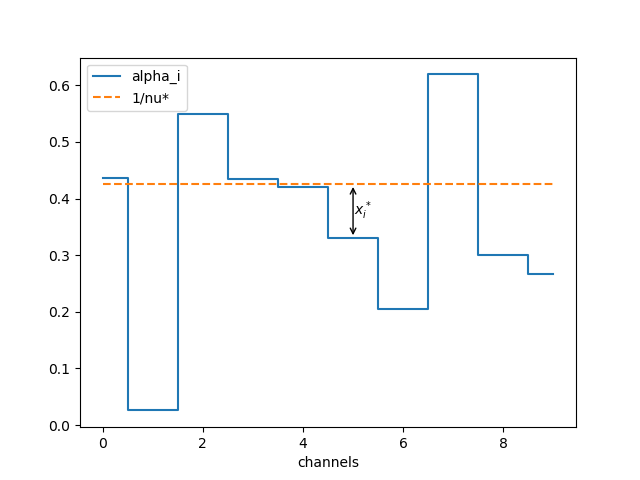
\includegraphics[width=8cm]{hinh_chuong5_duality/water_filling.png}
	\caption{Hình minh họa nghiệm của bài toán water filling.}
	\label{fig:descent}	
\end{figure}




\section{Ghi chú}
Các thuật ngữ sử dùng trong phần này:\\
\begin{tabular}{ll}
\textit{Thuật ngữ tiếng Việt:} 	& \textit{Thuật ngữ tiếng Anh:}\\
bài toán đối ngẫu		& dual problem\\
hàm đối ngẫu			& dual function\\
liên hợp				& conjugate\\
đối ngẫu yếu			& weak duality\\
đối ngẫu mạnh			& strong duality\\
điều kiện Slater		& Slater condition
\end{tabular}





\begin{thebibliography}{8}
\bibitem{boyd}
Boyd, Stephen, Stephen P. Boyd, and Lieven Vandenberghe. Convex optimization. Cambridge university press, 2004.

\bibitem{cmulectures}
Convex optimization lectures. Available at www.stat.cmu.edu/$\sim$ryantibs/convexopt/.
\end{thebibliography}
\end{document}
